\documentclass[10pt,letterpaper]{article} 
%\usepackage{tikz}
%\usepackage{tools}
\usepackage{amsmath,amssymb,geometry,graphicx,enumitem,caption,subcaption}
%\usefonttheme{serif}‎
%\usepackage{ptext}‎
%\usepackage{xepersian}
%\settextfont{B Nazanin}
\usepackage{lipsum}
\setlength{\parindent}{0pt}
\newcommand{\pf}{$\blacksquare$}
\newcommand{\Q}[1]{\textbf{Question #1)}}
\newcommand{\EX}{\Bbb E}
\newcommand{\nl}{\newline\newline}
\providecommand{\pic}[2]{
\begin{center}
\includegraphics[width=#2]{#1}
\end{center}
}
\begin{document}
\Large
\begin{center}
In the name of beauty

The 2nd problem set solution of Optical Networks course

\hrulefill
\end{center}
\Q1

\begin{enumerate}[label=\alph*)]
\item
False. As load balancing refers to traffic distribution among datasets, it is actually implemented in application layer.
\item
False. 3R-regeneration requires deploying transponders which imposes and OEO structure.
\item
False. If so, light would be more keen to leave the fiber than staying in it!
\item
False. They do reside at network edge.
\end{enumerate}

\Q2

\begin{enumerate}[label=\alph*.]
\item
$$
N_A=\sqrt{n_1^2-n_2^2}\approx0.12
$$
\item
$$
BL<\frac{n_2}{n_1^2}\frac{c}{\Delta}
$$
in which
$$
\Delta=1-\frac{n_2}{n_1}
$$
hence
$$
L_{max}\approx 6\text{km}
$$
\end{enumerate}

\Q3

\begin{equation}\begin{split}
&\text{Non-linear: } e^{j2\pi f_0t}\to e^{j2\pi f_0t}e^{j\gamma L}=e^{j2\pi f_0t+j\gamma L}
\\&
\text{Linear: } e^{j2\pi f_0t+j\gamma L}\to e^{j2\pi f_0t+j\gamma L}e^{j2\pi^2\beta_2Lf_0^2}
\\&
\text{Total Phase Rotation: }\gamma L+2\pi^2\beta_2Lf_0^2
\end{split}\end{equation}
%A link consisting of two equal spans interconnects two nodes as follows:
%\begin{figure}[ht]
%\centering
%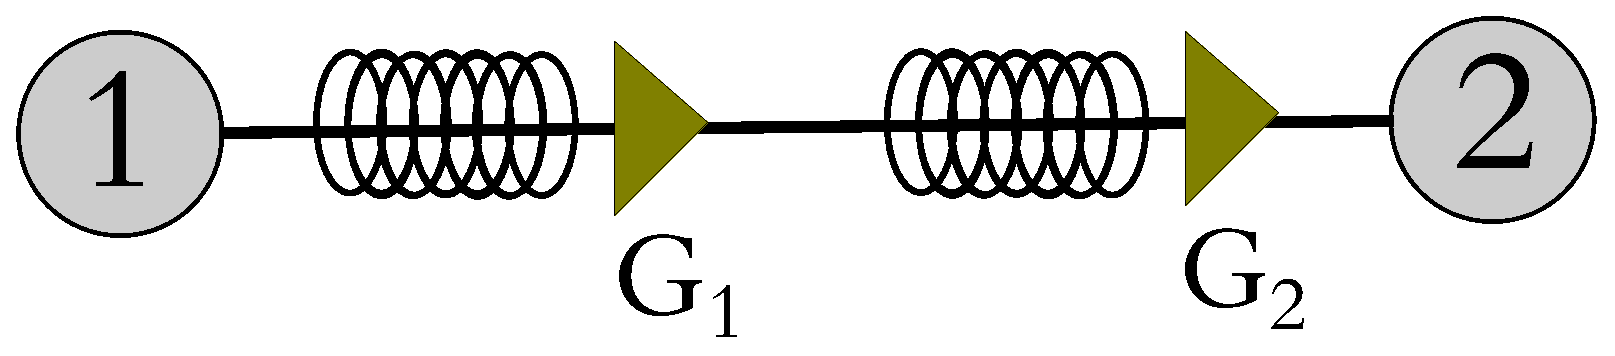
\includegraphics[scale=0.3]{PS2_P2P}
%\end{figure}
%
%Each span is constituted by a single-mode fiber (SMF) of length $L=100\text{km}$ and attenuation coefficient ($\alpha$) of $0.2\text{dB/km}$ and an EDFA. The power gains of the EDFAs are denoted by $G_1$ and $G_2$, the receiver bandwidth is $50\text{GHz}$ and each amplifer has a noise figure of $5\text{dB}$.
%\begin{enumerate}[label=\alph*)]
%\item
%For $G_1=13\text{dB}$ and $G_2=16\text{dB}$, calculate the total noise power at receiver.
%\item
%Assuming the receiver power sensitivity to be $0\text{dBu}$, with $G_1$ and $G_2$ take the same values of part a. Calculate the minimum power that should be launched into the link for a correct detection at receiver (sensitivity is the minimum power that turns on a device on its working point of operation).
%\end{enumerate}
%(Hints: The EDFA noise variance is obtained from
%$$
%\sigma_n^2=h\nu_\text{opt}GFW
%$$
%where
%$h=6.626\times 10^{-34}\text{J.sec}$ and $\nu_\text{opt}=194\text{THz}$. Note that all the scales are linear!
%
%The input power to the receiver is the summation of signal+noise powers.)
%
%\Q4
%
%Assume the same optical system of question 2. The amplifier gain $G_1$ is 10dB, but $G_2$ can arbitrarily vary within (0dB,100dB).
%
%\begin{enumerate}[label=\alph*)]
%\item
%How much is the maximum and minimum of achievable SNR at receiver? Assume the achievable SNR is defined as the ratio of signal power to noise variance at the input of receiver.
%\item
%Which one of either $G_1=10\text{dB},G_2=30\text{dB}$ or $G_1=30\text{dB},G_2=10\text{dB}$ is better from the QoS (quality-of-service) point of view (i.e., leads to more SNR)? What is the general reason of this?
%\end{enumerate}

\end{document}